\documentclass[11pt]{article}

\usepackage[margin=1in]{geometry}
\usepackage[T1]{fontenc}
\usepackage[utf8]{inputenc}
\usepackage{lmodern}
\usepackage{setspace}
\usepackage{amsmath, amssymb, amsthm}
\usepackage{booktabs}
\usepackage{graphicx}
\usepackage{float}
\usepackage{caption}
\usepackage{subcaption}
\usepackage{xcolor}
\usepackage{hyperref}
\usepackage{enumitem}

\onehalfspacing
\graphicspath{{figures/}}
\captionsetup{font=small}
\setlist{nosep,leftmargin=1.25em}
\setlength{\textfloatsep}{8pt plus 2pt minus 2pt}
\setlength{\floatsep}{8pt plus 2pt minus 2pt}

\title{Estimating Spillover Radius Under Latent Networks:\\A Design-Based Exposure-Mapping Simulation Study}
\author{Stefan Nicov, Albert Sveen, Feriel Terras \\ STAT 175 Final Project}
\date{\today}

\begin{document}
\maketitle

\begin{abstract}
This paper studies finite-sample recovery of a spillover radius when interference is mediated by a latent social network but the researcher observes only treatment, outcomes, covariates, and geographic locations. We build a simulation pipeline motivated by design-based exposure mapping. The data-generating process assigns units to locations, draws randomized treatment, constructs latent friendship structures, and generates outcomes through geographic or network-weighted exposure within a true radius. Our main methodological contribution is a predictive exposure-sufficiency criterion: for each candidate radius, fit a dose-response model using the geographic treated count and choose the radius with smallest residual mean squared error. This objective is a simple way to operationalize the idea that the correct exposure map should make outcomes measurable with respect to $g(W)$. The simulations show exact recovery under a correctly specified expected-Erdos-Renyi linear exposure model, but realistic errors under nonlinear saturated dose responses, noisy distances, clustered geography, and latent networks with distance decay, homophily, communities, or hubs. Overall, radius recovery is strongest when geographic exposure is a good sufficient summary of interference and weakest when influence is concentrated through special network positions or when the dose-response is too flat to identify local variation.
\end{abstract}

\section{Introduction}
Introduced by Sir David R. Cox in 1958, the non-interference assumption says that for each $j$, the treatment of others has no impact on the outcome for the jth individual, meaning that for each person, there are only two potential outcomes—one under treatment and one under non-treatment. And for good reason: had it not been for the non-interference assumption, for a study with n people, there would be $2^n$ potential outcomes per person which would be very difficult to keep track of \cite[p.~332]{blitzstein-shephard}. Simply put, the non-interference assumption collapses $Y_j(w_1,\dots,w_j, \dots, w_n)$ to $Y_j(w_j)$. 

Although greatly convenient and acceptable in some cases, this assumption breaks down when trying to model phenomena that rely on interaction between participants, including disease propagation and economic subsidies in a community. Naturally, these situations cannot ignore this non-interference assumption, and experimenters must consider how to incorporate these \emph{spillover effects}. A very natural and practical question is to understand how far out these \emph{spillover effects} extend, as this could inform quarantine legislation for outbreaks and quantify multiplier effects for economic policy intervention. 

A core challenge is that true spillovers may be mediated by unobserved networks. Though we are usually given geographic data in the form of zip codes and addresses, we do not observe the latent  networks in a community (such as friendship) that are responsible for disease propagation or economic subsidy disbursement. 

To recover this true radius of spillover effects $r_{\text{true}}$, we break this problem down into two stages.
\textcolor{red}{First, we implement a design-based radius estimator aligned with the exposure-mapping framework
of\textbf{has this paper been published yet?}, adapted to the setting where only geographic proximity is observed.} Second we present simulation evidence on finite-sample recovery of $r_{\text{true}}$ under a latent Erdos Renyi friendship network. Here, we also conduct a sensitivity analysis over different parameters including outcome noise, network sparsity via friendship probabilities, and treatment probabilities, isolating the conditions which most severerly distort recovery of $r_{\text{true}}$ and seeing when the estimator succeeds and when it breaks down. 

\section{Research Question and Contribution}

The project asks a narrow question: when the true interference process is generated by a latent network but the analyst observes only geography, when can a geographic exposure map recover the true radius of spillovers? This is a useful question for network inference because many applied settings have geographic coordinates, addresses, or zip codes, but do not have the actual friendship, communication, or economic interaction network that transmits spillovers.

The contribution is a simulation study that separates three mechanisms. First, if the outcome is truly measurable with respect to the observed geographic exposure map, radius recovery can be nearly exact. Second, if the exposure map is correct but the dose-response model is too simple, finite-sample recovery becomes noisy. Third, if the latent network changes which treated neighbors matter, the recovered radius may become an ``effective'' geographic radius rather than the structural cutoff.

\section{Simulation Design}

\subsection{Population and Geography}

Each simulation begins with $n$ units. In the baseline geography, units are placed independently and uniformly on a $150$ km by $150$ km square. We compute the Euclidean distance
\[
d_{ij}=\left\{(x_i-x_j)^2+(y_i-y_j)^2\right\}^{1/2}.
\]
Most scenarios use the true distance matrix as the observed distance matrix. In the noisy-distance robustness check, outcomes are generated using the true distances while the estimator uses perturbed observed distances.

We also study a two-cluster geography. Half of the units are centered in the left part of the square and half in the right part, with within-cluster standard deviation swept over several values. This creates a non-uniform distance distribution and tests whether the estimator is sensitive to spatial clustering.

\subsection{Treatment Assignment and Covariates}

Treatments are assigned independently as
\[
W_i\sim \text{Bernoulli}(\pi),
\]
with $\pi=0.5$ in the main simulations and a separate sweep over $\pi\in\{0.1,0.25,0.5,0.75,0.9\}$. Covariates include age, gender, education, race, and income. These covariates enter the outcome, and in the homophily scenario they also determine latent friendship probabilities.

\subsection{Latent Network and Exposure}

The latent adjacency matrix $A$ is generated but not observed by the estimator. We study several network models:
\begin{itemize}[leftmargin=1.25em]
    \item Erdos-Renyi: $A_{ij}\sim \text{Bernoulli}(p)$.
    \item Distance decay: $\Pr(A_{ij}=1)=\text{logit}^{-1}\{a-bd_{ij}/\text{median}(d)\}$.
    \item Covariate homophily: $\Pr(A_{ij}=1)$ increases with similarity in age, income, gender, education, and race.
    \item Stochastic block model: within-community edge probability $p_{in}$ and across-community probability $p_{out}$.
    \item Central hubs: $k$ hub nodes are connected to everyone while non-hub pairs connect with low probability.
\end{itemize}

The main estimand is the radius $r_{\text{true}}$ governing which geographic neighbors can contribute to spillovers. Define the geographic treated count
\[
C_i(r)=\sum_{j\neq i} W_j\mathbf{1}\{d_{ij}\le r\}.
\]
For the clean expected-Erdos-Renyi DGP, the spillover is
\[
S_i=pC_i(r_{\text{true}}).
\]
This case is intentionally favorable: the true outcome depends linearly on the same exposure summary used by the estimator.

For the main non-perfect simulations, we instead use a saturated response:
\[
S_i=1-\exp\{-\lambda p C_i(r_{\text{true}})\},
\]
with $\lambda=0.10$. This preserves the exposure-sufficiency condition $Y(W)=\widetilde{Y}(g(W))$ but makes the linear working model misspecified. For network-structured robustness checks, $p$ is replaced by pair-specific expected tie probabilities $p_{ij}$:
\[
S_i=1-\exp\left\{-\lambda\sum_{j\neq i}p_{ij}W_j\mathbf{1}\{d_{ij}\le r_{\text{true}}\}\right\}.
\]

\subsection{Outcome Model}

Outcomes are generated as
\[
Y_i=\alpha+X_i^\top\beta+\tau W_i+\gamma S_i+\epsilon_i,
\qquad
\epsilon_i\sim N(0,\sigma^2).
\]
The moderate baseline used for most robustness scenarios is
\[
n=1000,\qquad r_{\text{true}}=30,\qquad \gamma=1,\qquad \sigma^2=1,\qquad p=0.2.
\]

\subsection{Scenario Families}

The simulation design is organized so that each scenario changes one feature while holding the moderate baseline fixed. This makes failures interpretable: when estimates move, the change can be attributed to a specific source of weak identification or exposure misspecification.

\begin{table}[H]
    \centering
    \caption{Scenario families used in the Monte Carlo study.}
    \small
    \begin{tabular}{lll}
        \toprule
        Family & Parameter varied & Identification stress test \\
        \midrule
        Outcome noise & $\sigma^2$ & Signal-to-noise ratio \\
        Network density & ER $p$ & Number of relevant latent ties \\
        True radius & $r_{\text{true}}$ & Boundary and density effects \\
        Sample size & $n$ & Finite-sample instability \\
        Distance noise & noise in $d^{obs}_{ij}$ & Measurement error in exposure map \\
        Distance decay & decay strength & Weighted local ties vs. unweighted counts \\
        Homophily & similarity scale & Covariate-weighted latent friendship \\
        SBM & $p_{in}$ & Latent community structure \\
        Hubs & number of hubs $k$ & Concentrated network influence \\
        Two clusters & cluster spread & Non-uniform geography \\
        Treatment probability & $\pi$ & Exposure variation under design \\
        \bottomrule
    \end{tabular}
    \label{tab:scenario_families}
\end{table}

\section{Estimator}

\subsection{Exposure-Mapping Motivation}

The motivating exposure-mapping condition is that potential outcomes can be summarized by a lower-dimensional exposure:
\[
Y_i(W)=\widetilde{Y}_i(g_i(W;r)).
\]
This is the key conceptual reduction. Instead of modeling the full treatment vector $W\in\{0,1\}^n$, the analyst proposes an exposure map $g_i(W;r)$ and asks whether the potential outcome depends on $W$ only through that lower-dimensional summary. The unknown radius $r$ indexes a class of candidate exposure maps. In our setting, the researcher observes geography but not the latent network. The working exposure map is therefore the geographic treated count
\[
g_i(W;r)=C_i(r).
\]
If $r$ is too small, the exposure omits treated units that matter. If $r$ is too large, it includes treated units that should not matter. The estimation problem is therefore a model-selection problem over candidate exposure maps: choose the radius for which the induced exposure summary is most sufficient for outcomes.

\subsection{Original Moment-Based Approach}

The exposure-mapping framework can be turned into a design-based GMM estimator. The idea is to build functions of the treatment assignment, $\psi_m(W)$, and residualize them with respect to the candidate exposure map. For a candidate radius $r$, define moments of the form
\[
\eta_{m,i}(r)=\phi_m(Y_i)\,R_{i,r}\psi_m(W),
\qquad
R_{i,r}\psi_m(W)=\psi_m(W)-\widehat{\mathbb{E}}\{\psi_m(W)\mid W_i,g_i(W;r)\}.
\]
When $g_i(W;r)$ is the correct exposure map, residualized treatment functions should be orthogonal to outcomes under the known experimental design. In implementation, we kept the outcome transform literal, $\phi_m(Y_i)=Y_i$, and evaluated the conditional expectation either by placebo treatment redraws or, for Bernoulli treated-count cases, by exact analytical conditioning. This moment construction is attractive because it is fully design-based: the only randomness used for residualization comes from the known assignment mechanism.

\subsection{Our Proposed Predictive Sufficiency Criterion}

Our main contribution is to propose a simpler estimator that targets the same exposure-sufficiency idea more directly. Rather than choosing instruments $\psi_m$ and estimating many conditional expectations, we ask a predictive question: for which candidate radius does $g_i(W;r)$ make $Y_i$ easiest to explain?

For each candidate radius $r$ on a discrete grid, we fit
\[
Y_i=a_r+b_rW_i+c_rg_i(W;r)+u_{ir},
\]
and compute
\[
Q(r)=\frac{1}{n}\sum_{i=1}^n \hat u_{ir}^2.
\]
The estimate is
\[
\hat r=\arg\min_r Q(r).
\]
This criterion is a predictive operationalization of the same exposure-sufficiency condition. If $g_i(W;r)$ is sufficient, then conditioning on it should remove systematic dependence of $Y_i$ on other parts of the assignment vector. The MSE criterion chooses the radius whose exposure map leaves the least unexplained outcome variation. The estimator is also easy to implement: it requires only observed outcomes, treatment, locations, and a regression routine.

\subsection{Why the MSE Criterion Recovers the Radius}

The following population argument explains why the criterion works in the clean case.

\textbf{Proposition.} Suppose the true outcome satisfies
\[
Y_i=\alpha+\tau W_i+h\{C_i(r_0)\}+\epsilon_i,
\qquad
\mathbb{E}[\epsilon_i\mid W, X]=0,
\]
where $r_0$ is the true radius. Suppose also that the working dose-response class contains the true function $h$ and that, for any $r\ne r_0$, $C_i(r_0)$ is not measurable with respect to $(W_i,C_i(r))$. Then the population prediction risk
\[
R(r)=\inf_f \mathbb{E}\left[\{Y_i-f(W_i,C_i(r))\}^2\right]
\]
is uniquely minimized at $r=r_0$.

\textit{Sketch.} For any candidate $r$, the best predictor under squared loss is the conditional expectation,
\[
f_r^\star(W_i,C_i(r))=\mathbb{E}[Y_i\mid W_i,C_i(r)].
\]
At $r=r_0$, this conditional expectation equals $\alpha+\tau W_i+h\{C_i(r_0)\}$, so the remaining risk is only the irreducible noise variance $\mathbb{E}[\epsilon_i^2]$. For $r\ne r_0$, the conditioning variables do not contain the true exposure $C_i(r_0)$. The best predictor must average over omitted variation in $h\{C_i(r_0)\}$, adding a positive conditional-variance term:
\[
R(r)=\mathbb{E}[\epsilon_i^2]+\mathbb{E}\!\left[\operatorname{Var}\{h(C_i(r_0))\mid W_i,C_i(r)\}\right].
\]
By the non-measurability assumption, this second term is positive for incorrect radii, so the risk is minimized at $r_0$.

Our implemented estimator uses a linear working approximation, $f(W_i,C_i(r))=a+bW_i+cC_i(r)$, so the finite-sample simulations also study what happens when the true $h$ is nonlinear and the working class is imperfect. This is why the clean linear DGP recovers exactly, while the saturated DGP produces informative but non-perfect recovery.

\section{Results}

\subsection{Correct Specification Versus Saturated Dose Response}

The clean expected-Erdos-Renyi linear DGP is almost exactly matched to the estimator, and it recovers $r_{\text{true}}=30$ across the noise and network-density sweeps. This is a sanity check: when the outcome is linear in the observed exposure map, the radius is identified by predictive fit.

The saturated DGP is more realistic. It still satisfies exposure sufficiency, but the working linear dose-response is too simple. Figure~\ref{fig:specification} shows that this change alone turns perfect recovery into noisy finite-sample recovery as outcome noise increases.

\begin{figure}[H]
    \centering
    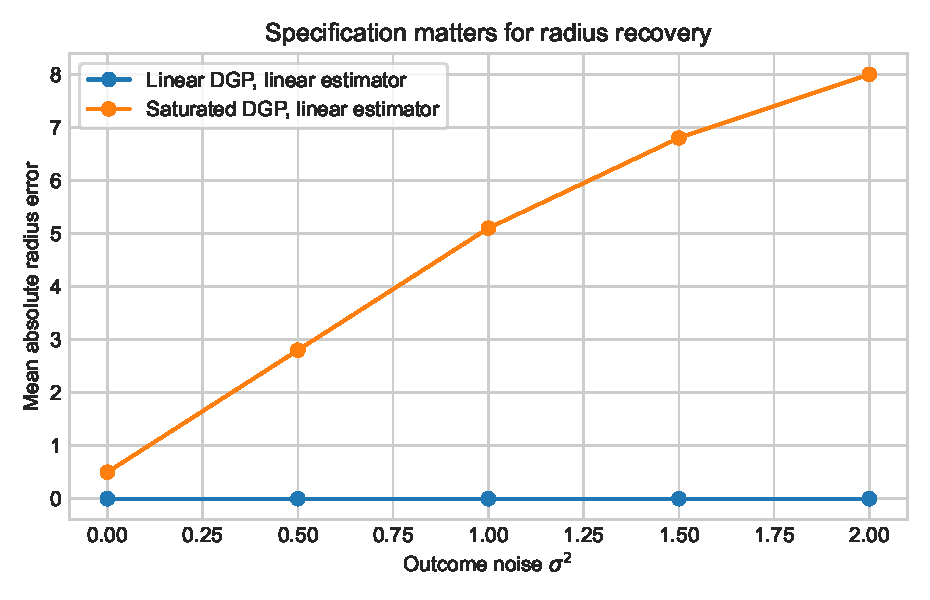
\includegraphics[width=0.72\textwidth]{specification_noise_comparison.pdf}
    \caption{Mean absolute radius error under a correctly specified linear expected-Erdos-Renyi DGP and a nonlinear saturated DGP. The estimator is linear in both cases.}
    \label{fig:specification}
\end{figure}

\subsection{Main Parameter Sweeps}

Figure~\ref{fig:main_sweeps} summarizes the main saturated-DGP sweeps. Recovery is stable under moderate noise, moderate network density, and sample sizes around $n=1000$ or larger. It is less stable at very low or high network density, at small sample sizes, and at extreme true radii. These patterns are consistent with the amount of useful local exposure variation available to the estimator.

Figure~\ref{fig:main_recovery} complements the error plot by showing the direction of the estimates. The $r_{\text{true}}$ sweep is especially informative: middle radii are easiest, while small and large cutoffs are harder because the exposure count changes less distinctly around the boundary. The $n$ sweep shows the expected finite-sample pattern: median recovery is poor for $n=100$ and $n=200$, then stabilizes near $30$ once the sample reaches roughly $1000$ units.

\begin{figure}[H]
    \centering
    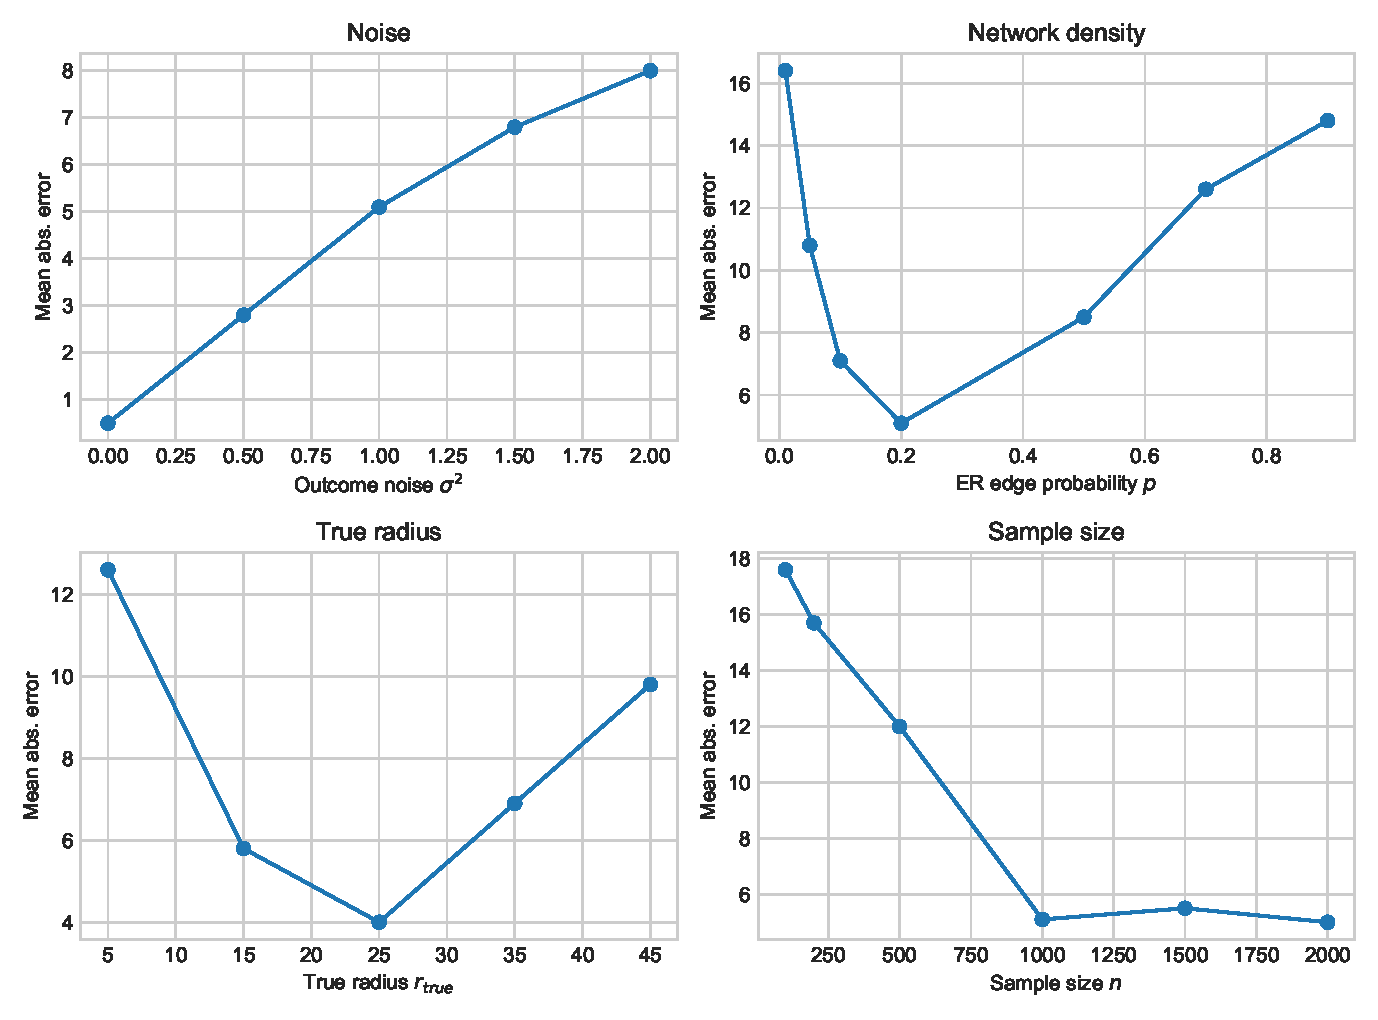
\includegraphics[width=0.88\textwidth]{main_saturated_sweeps.pdf}
    \caption{Main parameter sweeps under the saturated DGP: outcome noise, ER edge probability, true radius, and sample size.}
    \label{fig:main_sweeps}
\end{figure}

\begin{figure}[H]
    \centering
    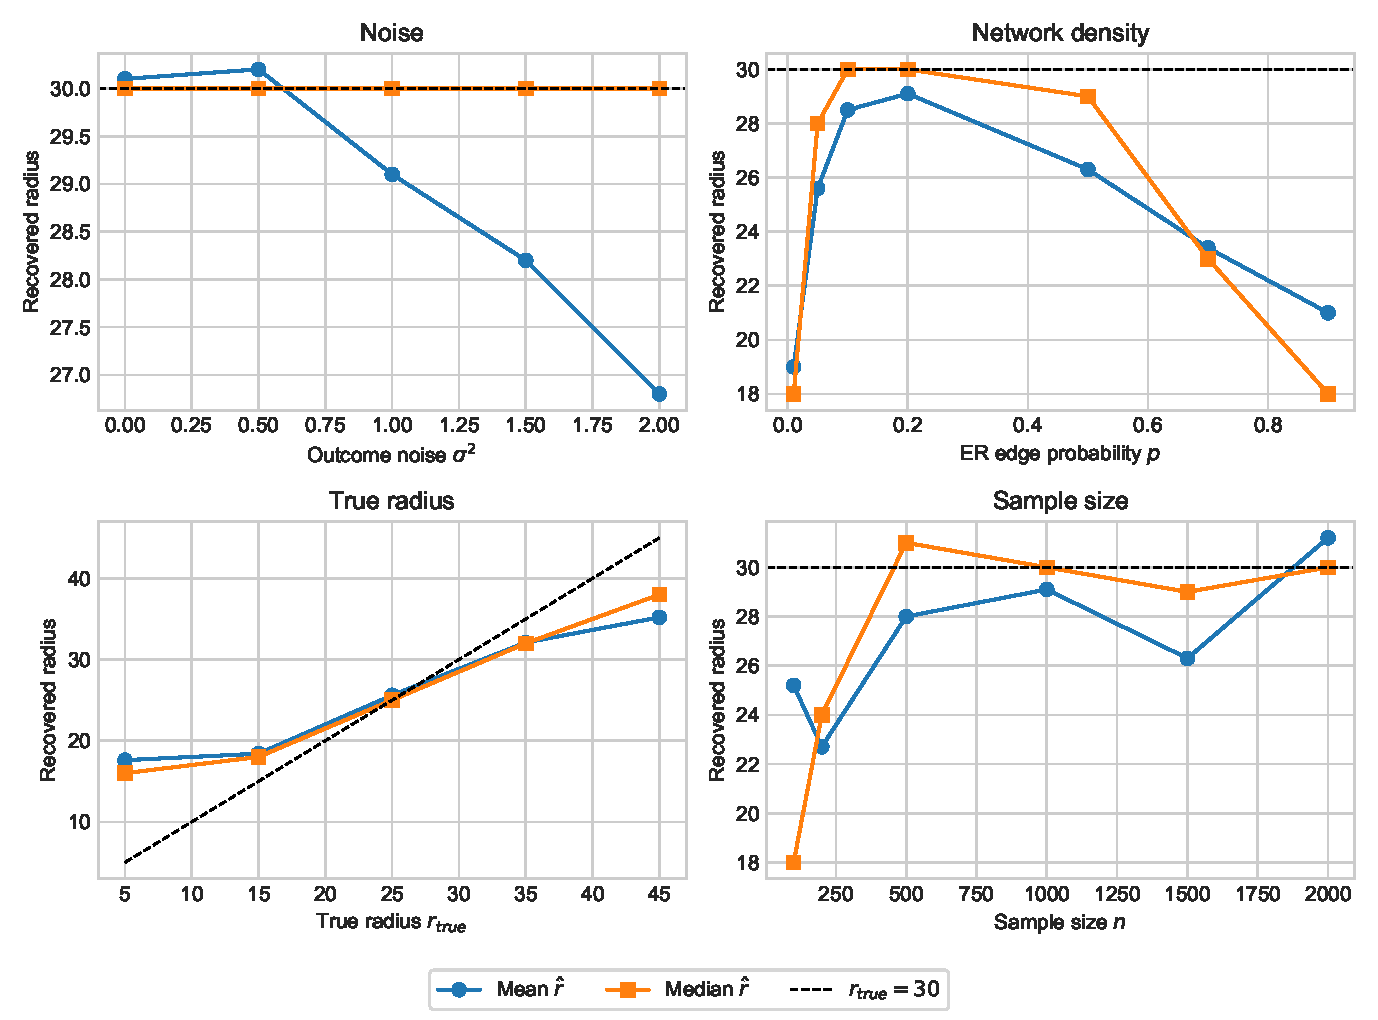
\includegraphics[width=0.82\textwidth]{main_recovery_levels.pdf}
    \caption{Mean and median recovered radii for the main saturated-DGP sweeps. Dashed lines mark the true radius, or the identity line for the $r_{\text{true}}$ sweep.}
    \label{fig:main_recovery}
\end{figure}

\begin{table}[H]
    \centering
    \caption{Selected saturated-DGP Monte Carlo results. Each row reports 20 seeds.}
    \begin{tabular}{lcccc}
        \toprule
        Sweep & Setting & Mean $\hat r$ & Median $\hat r$ & Mean $|\hat r-r_{\text{true}}|$ \\
        \midrule
        Noise & $\sigma^2=1$ & 29.1 & 30.0 & 5.1 \\
        Network density & $p=0.2$ & 29.1 & 30.0 & 5.1 \\
        True radius & $r_{\text{true}}=25$ & 25.6 & 25.0 & 4.0 \\
        Sample size & $n=1000$ & 29.1 & 30.0 & 5.1 \\
        Treatment probability & $\pi=0.25$ & 28.8 & 30.0 & 4.6 \\
        \bottomrule
    \end{tabular}
    \label{tab:selected}
\end{table}

\subsection{Latent Network Robustness}

Figure~\ref{fig:network} studies latent networks that are not simple ER graphs. Distance-decay networks tend to recover a smaller effective radius because closer treated units receive more weight even inside the true cutoff. Homophily and SBM structures improve as signal strength increases, but the estimator still ignores covariate similarity and community labels. Hub networks are a strong failure mode: a few central nodes dominate exposure, so unweighted geographic treated counts become a poor proxy for actual influence.

The network scenarios are useful because they distinguish two reasons geographic exposure can fail. In distance-decay networks, geography is still relevant, but the unweighted count is too crude: all treated neighbors inside $r$ receive equal weight even though the DGP gives more influence to closer neighbors. In hub networks, the problem is different: the relevant information is not only where treated units are, but whether treated units occupy special positions in the latent network. This explains why increasing the number of hubs raises the correlation between true spillover and outcome but does not make radius recovery reliable.

\begin{figure}[H]
    \centering
    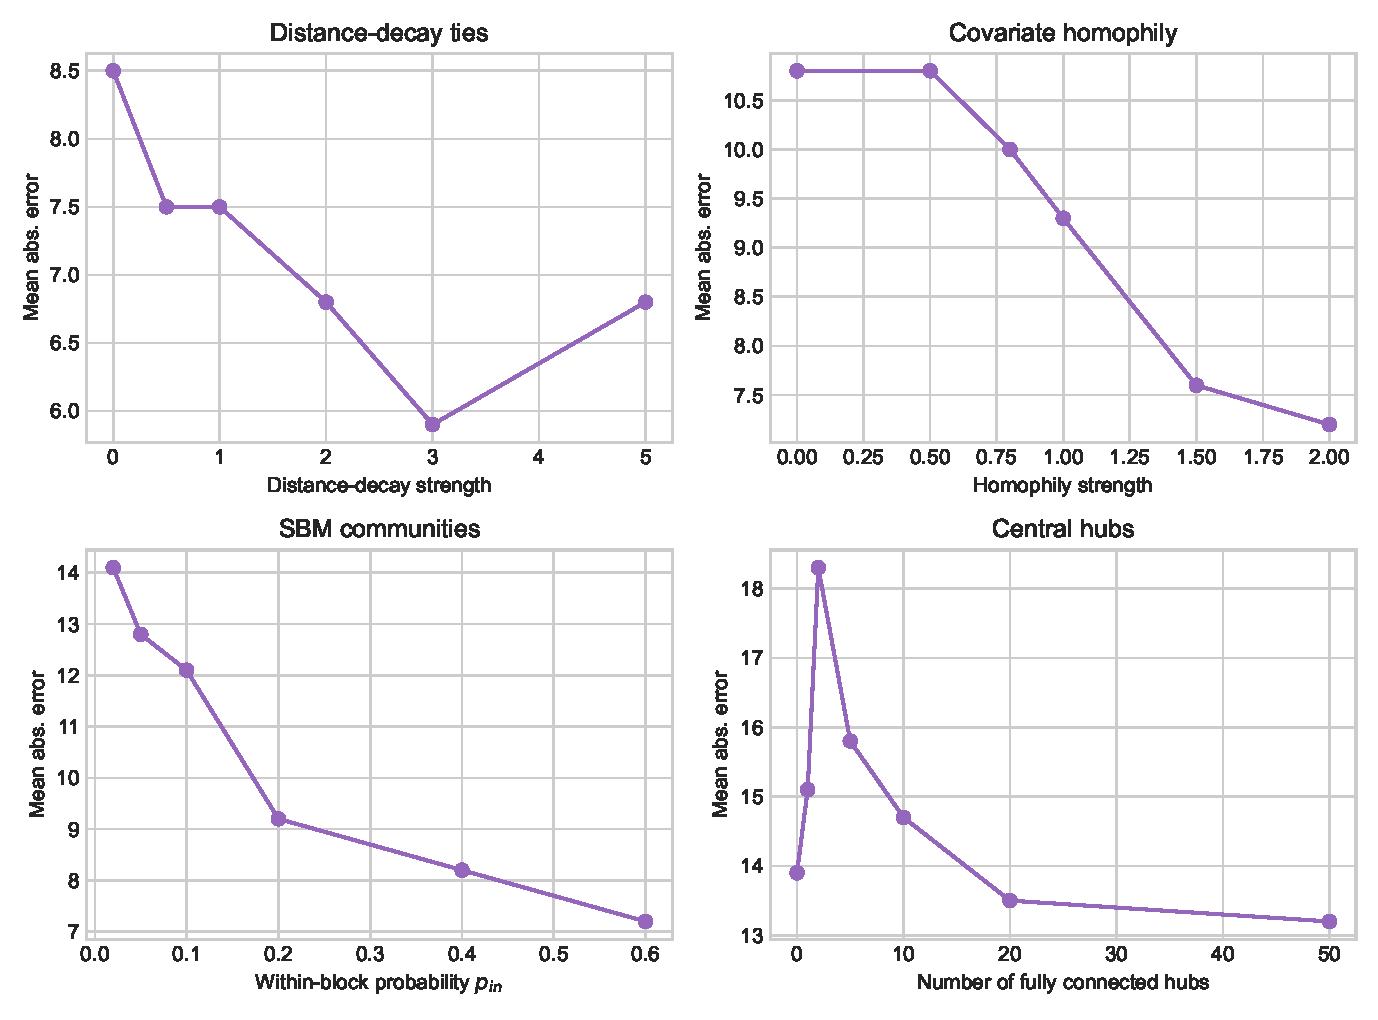
\includegraphics[width=0.92\textwidth]{latent_network_robustness.pdf}
    \caption{Robustness to latent network structure. The estimator does not observe the network and uses unweighted geographic treated counts.}
    \label{fig:network}
\end{figure}

\subsection{Measurement, Geography, and Design Robustness}

Figure~\ref{fig:design_geo} reports additional robustness checks. Noisy observed distances increase dispersion because the estimator forms exposure maps using a corrupted proxy for the true distance matrix. Two-cluster geography makes the objective noisier and can push estimates upward, especially when clusters are tight enough that many units have similar local exposure counts. Treatment probabilities near $0.25$ to $0.5$ perform best, while very low or high assignment probabilities reduce useful exposure variation.

These scenarios are closest to practical design concerns. Distance measurement error does not change the true spillover rule, but it changes the analyst's exposure map. Clustered geography changes the distribution of distances and can make multiple candidate radii produce similar exposure counts. Extreme treatment probabilities reduce design variation: when almost nobody or almost everybody is treated, local treated counts become less informative about the radius.

\begin{figure}[H]
    \centering
    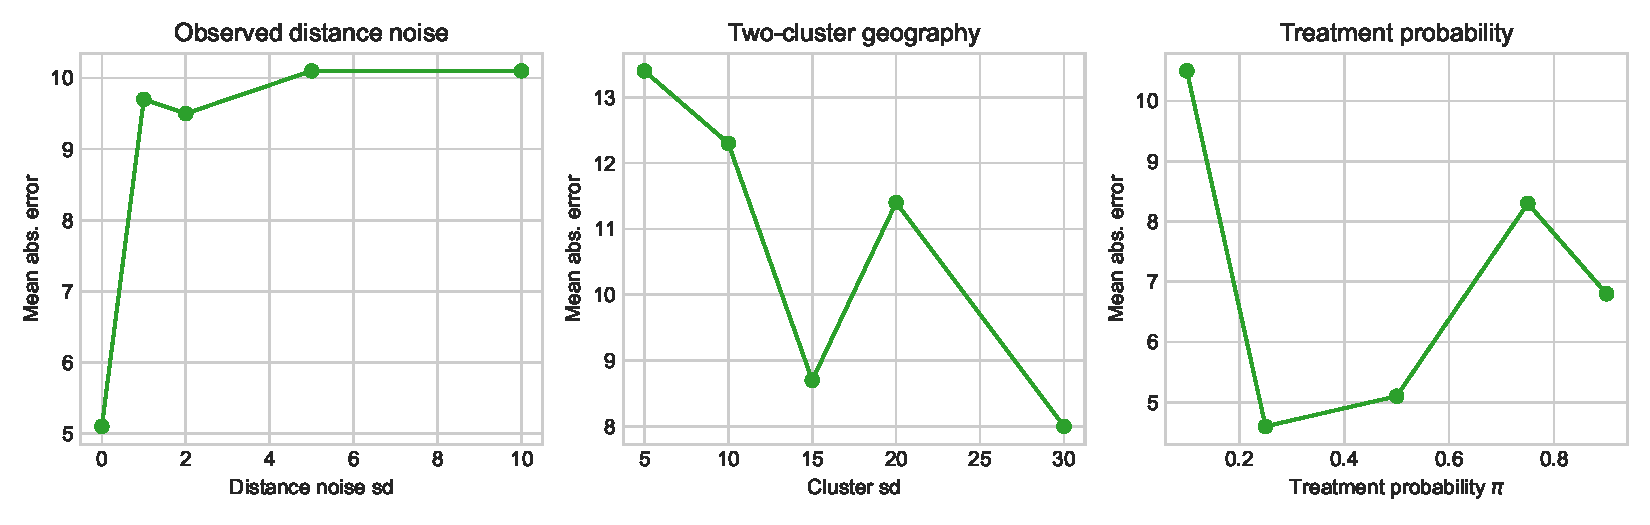
\includegraphics[width=0.95\textwidth]{design_geography_robustness.pdf}
    \caption{Robustness to observed distance noise, clustered geography, and treatment probability.}
    \label{fig:design_geo}
\end{figure}

\section{Discussion}

The main lesson is that exposure sufficiency has two layers. First, the chosen exposure map must contain the relevant treatment information. Second, the estimator must approximate the dose-response well enough to exploit that information. The clean linear DGP satisfies both conditions and produces exact recovery. The saturated DGP satisfies the first condition but weakens the second, producing realistic errors without abandoning the theoretical exposure-mapping idea.

The latent network scenarios show when geographic exposure is credible as a proxy. If latent ties are roughly exchangeable within geography, the geographic count can recover the true radius. If influence is weighted toward closer neighbors, specific communities, or hubs, the radius estimate can become an effective summary rather than the structural cutoff. This distinction is substantively important: a policy analyst might estimate a smaller radius not because spillovers cannot occur beyond it, but because most influential pathways are concentrated locally or through special nodes.

The project also illustrates a methodological tradeoff. The moment-based GMM construction is close to the design-based theory and avoids modeling the outcome regression directly, but it requires choosing a useful dictionary of treatment functions and estimating conditional expectations. The predictive criterion is less elaborate and easier to implement: it asks directly whether the proposed exposure map is sufficient for outcome prediction. In this sense, the two approaches are complementary. GMM provides a design-based orthogonality route, while the MSE objective provides a transparent sufficiency-testing route.

For applied work, the results suggest three diagnostics. First, inspect whether the objective has a clear minimum or is flat over a range of radii. Second, check sensitivity to plausible exposure transformations, such as nonlinear or saturated dose responses. Third, treat disagreement across network-robustness scenarios as evidence that the estimated radius is an effective geographic summary rather than a literal social-interaction cutoff.

\section{Conclusion}

We studied radius recovery when interference is mediated by latent networks but only geography is observed. A geographic exposure map can recover the true radius when it is sufficiently aligned with the true spillover process. Recovery degrades in informative ways under nonlinear dose responses, noisy distances, clustered geography, extreme treatment probabilities, and latent network structures that concentrate influence. These results suggest that estimating spillover radius is feasible, but the interpretation of $\hat r$ depends strongly on whether observed geography is a sufficient proxy for the latent interaction network.

\appendix

\section{Reproducibility Notes}

All reported simulations are generated from the config-driven pipeline in \texttt{simulations/}. Each scenario has its own folder under \texttt{simulations/scenarios/}, with timestamped output directories containing per-seed results, aggregate summaries, generated datasets, and diagnostic plots. Most Monte Carlo summaries use 20 seeds. The main report figures are generated from the aggregate CSV files and stored in \texttt{final\_report/figures/}.

\section{Scenario Inventory}

The main scenarios used in this report are:
\begin{itemize}[leftmargin=1.25em]
    \item \texttt{scenario\_20}: linear expected-ER noise sweep with $\gamma=1$.
    \item \texttt{scenario\_21}: saturated expected-ER noise sweep.
    \item \texttt{scenario\_22}: saturated expected-ER network-density sweep.
    \item \texttt{scenario\_23}: saturated expected-ER true-radius sweep.
    \item \texttt{scenario\_24}: saturated expected-ER sample-size sweep.
    \item \texttt{scenario\_25}: observed distance-noise sweep.
    \item \texttt{scenario\_26}: distance-decay latent network sweep.
    \item \texttt{scenario\_27}: covariate-homophily latent network sweep.
    \item \texttt{scenario\_28}: SBM community sweep.
    \item \texttt{scenario\_29}: central-hub latent network sweep.
    \item \texttt{scenario\_30}: two-cluster geography sweep.
    \item \texttt{scenario\_31}: treatment-probability sweep.
\end{itemize}

\section{Additional Result Ranges}

\begin{table}[H]
    \centering
    \caption{Range of mean absolute error across major robustness sweeps.}
    \begin{tabular}{lcc}
        \toprule
        Sweep & Minimum mean abs. error & Maximum mean abs. error \\
        \midrule
        Saturated noise & 0.5 & 8.0 \\
        Saturated ER density & 5.1 & 16.4 \\
        Saturated true radius & 4.0 & 12.6 \\
        Saturated sample size & 5.0 & 17.6 \\
        Distance measurement error & 5.1 & 10.1 \\
        Distance-decay network & 5.9 & 8.5 \\
        Covariate homophily network & 7.2 & 10.8 \\
        SBM communities & 7.2 & 14.1 \\
        Central hubs & 13.2 & 18.3 \\
        Two-cluster geography & 8.0 & 13.4 \\
        Treatment probability & 4.6 & 10.5 \\
        \bottomrule
    \end{tabular}
\end{table}

\section{Additional Diagnostic Figures}

\begin{figure}[H]
    \centering
    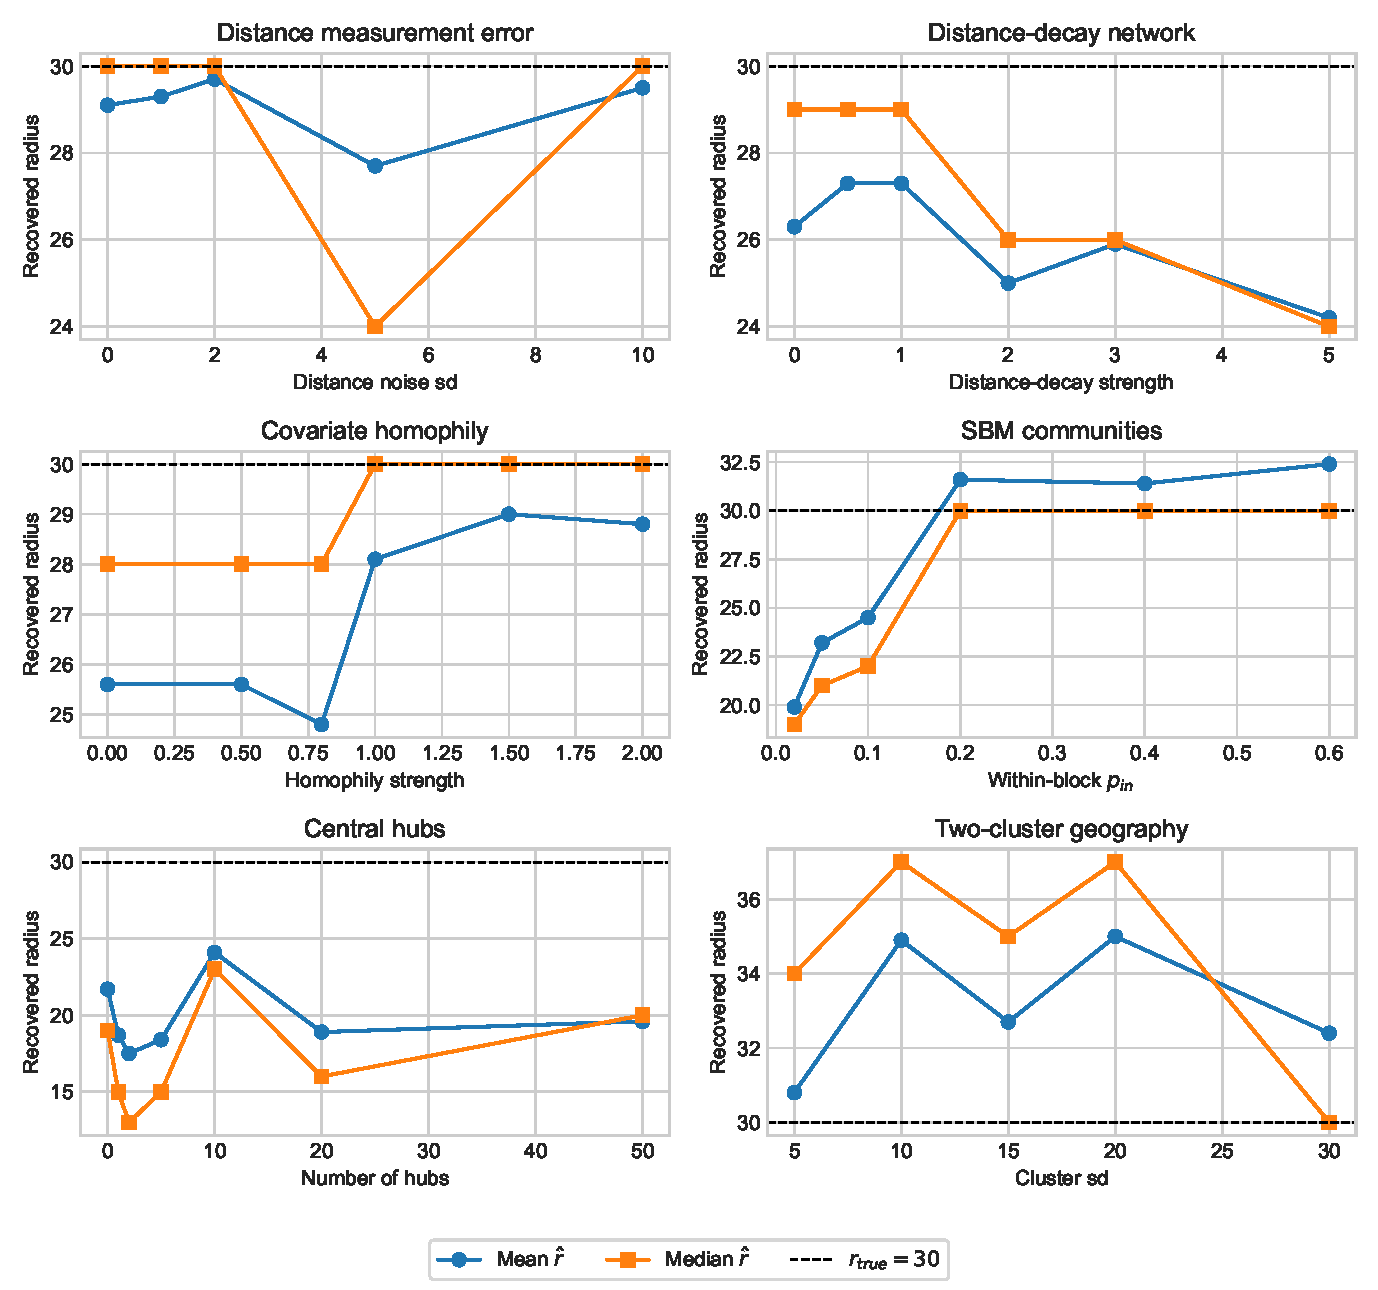
\includegraphics[width=0.82\textwidth]{robustness_recovery_levels.pdf}
    \caption{Mean and median recovered radii across robustness sweeps. The dashed line marks $r_{\text{true}}=30$.}
\end{figure}

\begin{figure}[H]
    \centering
    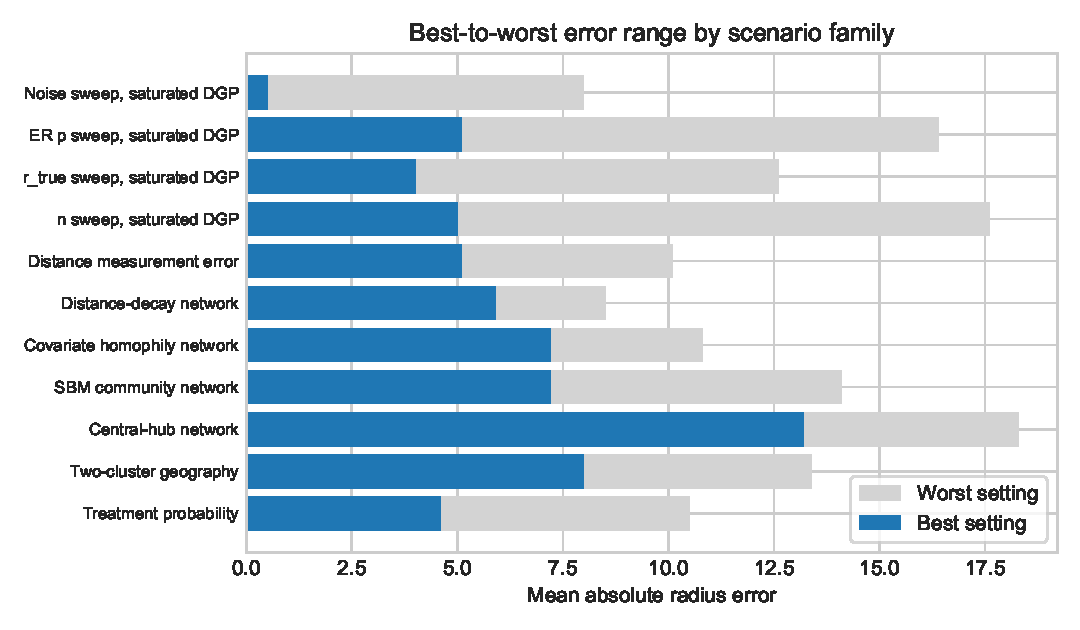
\includegraphics[width=0.78\textwidth]{scenario_error_ranges.pdf}
    \caption{Best-to-worst mean absolute radius error across scenario families. Hubs, low-density SBM, small samples, and clustered geography create the largest errors.}
\end{figure}

\begin{thebibliography}{9}

\bibitem{blitzstein-shephard}
Joseph K. Blitzstein and Neil Shephard,
\textit{Introduction to Statistics: Inference, Description, Prediction, and Causality},
STAT 111 course text, 2025.

\bibitem{cox1958}
David R. Cox,
\textit{Planning of Experiments},
Wiley, 1958.

\bibitem{aronow-samii}
Peter M. Aronow and Cyrus Samii,
Estimating average causal effects under general interference,
\textit{Annals of Applied Statistics}, 11(4):1912--1947, 2017.

\end{thebibliography}

\end{document}
